% ============================================================================
% CHAPTER 1 --- OFDM SYSTEM MODEL AND CLASSICAL PAPR REDUCTION TECHNIQUES
% ============================================================================
\chapter{OFDM System Model and Classical PAPR Reduction Techniques}
\label{ch:ofdm_papr}

This chapter presents the Orthogonal Frequency-Division Multiplexing (OFDM) signal model and defines the Peak-to-Average Power Ratio (PAPR) problem that motivates the machine-learning approaches studied in subsequent chapters. A concise survey of classical PAPR reduction techniques is provided, covering signal distortion methods and signal scrambling methods, with particular attention to Selected Mapping (SLM) as the primary baseline for the deep learning system introduced in Chapter~\ref{ch:prnet}.


% ----------------------------------------------------------------------------
\section{OFDM Signal Model}
\label{sec:ofdm_model}
% ----------------------------------------------------------------------------

Orthogonal Frequency-Division Multiplexing divides a wideband channel into $N$ narrowband, orthogonal subcarriers.  Each subcarrier carries one modulated symbol from a constellation such as QPSK or $M$-QAM.  The modulation and demodulation operations are efficiently implemented via the Inverse Fast Fourier Transform (IFFT) and Fast Fourier Transform (FFT), respectively.

\begin{figure}[H]
    \centering
    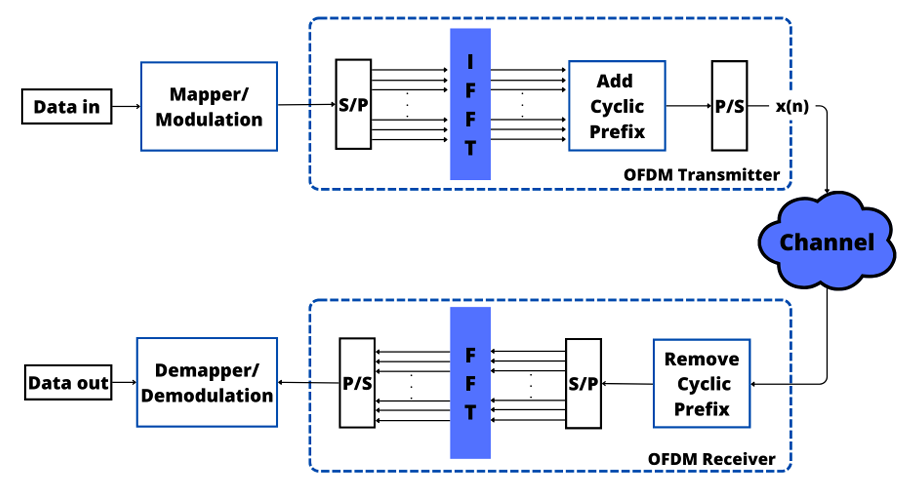
\includegraphics[width=0.70\linewidth]{Figures/OFDM_Refresher/ofdm_block_diagram.png}
    \caption{Block diagram of a baseband OFDM transmitter and receiver. The transmitter maps data onto $N$ subcarriers via an $N$-point IFFT, adds a cyclic prefix (CP), and transmits the time-domain signal.  The receiver removes the CP and applies an $N$-point FFT to recover the frequency-domain symbols.}
\end{figure}


\subsection{Subcarrier Modulation via the IFFT}

Let the frequency-domain data symbol vector after constellation mapping be
\begin{equation*}
    \bm{X} = \bigl[X[0],\; X[1],\; \dots,\; X[N-1]\bigr]^T,
\end{equation*}
where $X[k]$ is the complex symbol transmitted on the $k$-th subcarrier and $N$ is the total number of subcarriers.  The time-domain OFDM signal is obtained by applying the $N$-point IFFT:
\begin{keyresult}
\begin{equation}
    x[n] = \frac{1}{\sqrt{N}} \sum_{k=0}^{N-1} X[k] \, e^{\,j2\pi kn/N},
    \qquad n = 0,\, 1,\, \dots,\, N-1.
\end{equation}
\end{keyresult}

The $1/\!\sqrt{N}$ normalization preserves signal energy between the frequency and time domains (Parseval's theorem).  At the receiver, the frequency-domain symbols are recovered by the complementary FFT operation:
\begin{keyresult}
\begin{equation}
    X[k] = \frac{1}{\sqrt{N}} \sum_{n=0}^{N-1} x[n] \, e^{-\,j2\pi kn/N},
    \qquad k = 0,\, 1,\, \dots,\, N-1.
\end{equation}
\end{keyresult}


\subsection{Cyclic Prefix}

Before transmission, a \textbf{Cyclic Prefix (CP)} of length $N_{\mathrm{cp}}$ samples is prepended to each OFDM symbol by copying the last $N_{\mathrm{cp}}$ samples of the IFFT output to the front.  The CP serves two purposes:
\begin{enumerate}
    \item \textbf{ISI elimination:} provided $N_{\mathrm{cp}}$ exceeds the maximum channel delay spread, the CP absorbs all multipath echoes from the previous symbol.
    \item \textbf{Circular convolution:} the CP converts the linear convolution with the channel into a circular convolution, enabling single-tap equalization in the frequency domain via the FFT.
\end{enumerate}


\subsection{Spectral Efficiency}

\begin{figure}[H]
    \centering
    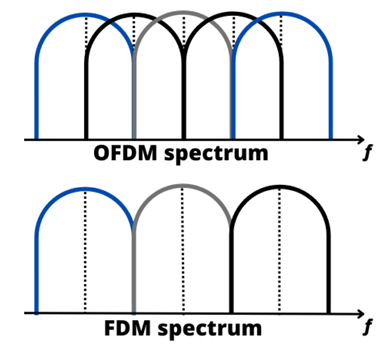
\includegraphics[width=0.45\linewidth]{Figures/OFDM_Refresher/fdm_vs_ofdm_spectrum.png}
    \caption{Spectrum comparison between conventional Frequency-Division Multiplexing (FDM) and OFDM.  In FDM, guard bands between channels reduce spectral efficiency.  In OFDM, orthogonal subcarriers overlap without mutual interference.}
\end{figure}

OFDM subcarriers are spaced at exactly $\Delta f = 1/T_s$, where $T_s$ is the useful symbol duration.  At every subcarrier's centre frequency, all other subcarriers have a spectral null, ensuring zero mutual interference and significantly higher spectral efficiency compared to conventional FDM.


% ----------------------------------------------------------------------------
\section{Peak-to-Average Power Ratio}
\label{sec:papr}
% ----------------------------------------------------------------------------

\subsection{Definition}

The time-domain OFDM signal is the superposition of $N$ independently modulated complex exponentials.  When these subcarrier contributions align constructively at certain time instants, large amplitude peaks occur.  The severity of this phenomenon is quantified by the \textbf{Peak-to-Average Power Ratio (PAPR)}:
\begin{keyresult}
\begin{equation}
    \mathrm{PAPR}\bigl(\bm{x}\bigr)
    = \frac{\displaystyle\max_{0 \le n \le N-1}\bigl|x[n]\bigr|^{2}}
           {E\Bigl[\bigl|x[n]\bigr|^{2}\Bigr]},
\end{equation}
\end{keyresult}
where the numerator is the peak instantaneous power and the denominator is the average power of the OFDM symbol.  The theoretical worst-case PAPR for $N$ subcarriers is $10\log_{10}(N)$~dB, which occurs when all subcarriers align perfectly in phase.


\subsection{CCDF Performance Metric}

Since PAPR varies from one OFDM symbol to the next, it is characterised statistically using the \textbf{Complementary Cumulative Distribution Function (CCDF)}:
\begin{equation*}
    \mathrm{CCDF}_{\mathrm{PAPR}}
    = \Pr\bigl(\mathrm{PAPR} > \mathrm{PAPR}_0\bigr),
\end{equation*}
where $\mathrm{PAPR}_0$ is a given threshold. For $N$ subcarriers with independent, identically distributed symbols and Nyquist-rate sampling, the CCDF can be approximated as:
\begin{keyresult}
\begin{equation}
    \Pr\bigl(\mathrm{PAPR} \ge \mathrm{PAPR}_0\bigr)
    \approx 1 - \bigl(1 - e^{-\mathrm{PAPR}_0}\bigr)^{N}.
\end{equation}
\end{keyresult}

A PAPR reduction technique shifts the CCDF curve to the left, indicating that high-PAPR events become statistically less likely.

\begin{figure}[H]
    \centering
    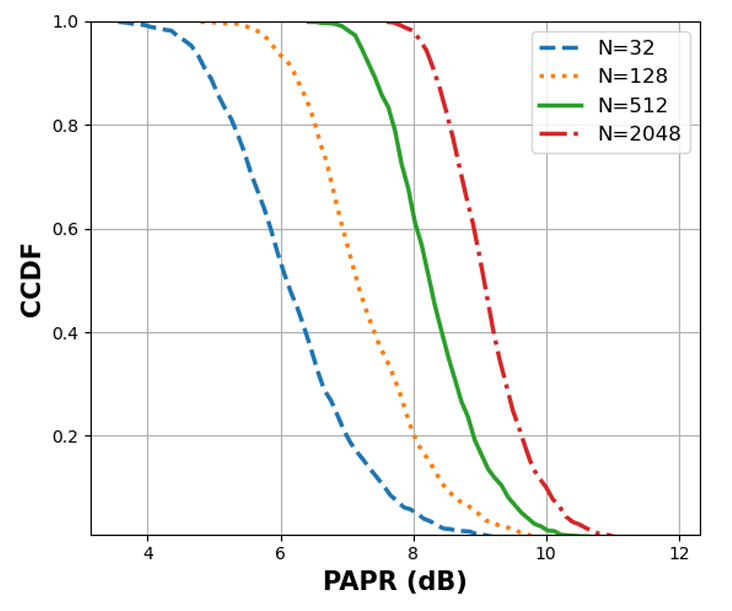
\includegraphics[width=0.55\linewidth]{Figures/OFDM_Refresher/ccdf_subcarriers.png}
    \caption{CCDF of PAPR for different numbers of subcarriers ($N = 32, 128, 512, 2048$) with 16-QAM modulation. As $N$ increases, the PAPR distribution shifts to the right, confirming that more subcarriers lead to higher PAPR.}
\end{figure}


\subsection{Power Amplifier Nonlinearity}

High PAPR has direct consequences for the \textbf{High-Power Amplifier (HPA)} at the transmitter.  Every power amplifier has a saturation region: when the input signal exceeds a certain amplitude, the output clips or compresses, introducing nonlinear distortion.  To avoid entering this nonlinear zone, the HPA must operate with sufficient \textbf{Input Back-Off (IBO)}:
\begin{equation*}
    \mathrm{IBO\;(dB)} = 10\log_{10}\!\left(\frac{P_{\mathrm{sat}}}{P_{\mathrm{avg}}}\right),
\end{equation*}
where $P_{\mathrm{sat}}$ is the amplifier's saturation power and $P_{\mathrm{avg}}$ is the average input signal power.  For an OFDM signal with $\mathrm{PAPR} = 12$~dB, the IBO must be at least 12~dB, meaning the amplifier operates far below its maximum capacity.  This directly reduces power efficiency and increases hardware complexity.

Reducing PAPR by even 3--4~dB translates to a significant improvement in HPA efficiency, reduced heat dissipation, and lower deployment costs, making PAPR reduction one of the most active research areas in OFDM system design.


% ----------------------------------------------------------------------------
\section{Classical PAPR Reduction Techniques}
\label{sec:classical_papr}
% ----------------------------------------------------------------------------

Classical PAPR reduction techniques can be broadly classified into \textbf{signal distortion} methods, which introduce controlled modifications to the transmitted signal, and \textbf{signal scrambling} methods, which generate alternative signal representations without distortion.


\subsection{Signal Distortion Techniques}

\paragraph{Clipping and Filtering.}
The simplest approach: any signal sample exceeding a threshold $A$ is clipped to that threshold.  Filtering is subsequently applied to suppress out-of-band spectral regrowth.  The clipped signal is given by:
\begin{equation*}
    x'[n] =
    \begin{cases}
        x[n], & |x[n]| \le A, \\[4pt]
        \dfrac{A}{|x[n]|}\, x[n], & |x[n]| > A,
    \end{cases}
\end{equation*}
where $A = \mathrm{CR}\cdot\sqrt{P_{\mathrm{avg}}}$ and $\mathrm{CR}$ is the clipping ratio.

\begin{figure}[H]
    \centering
    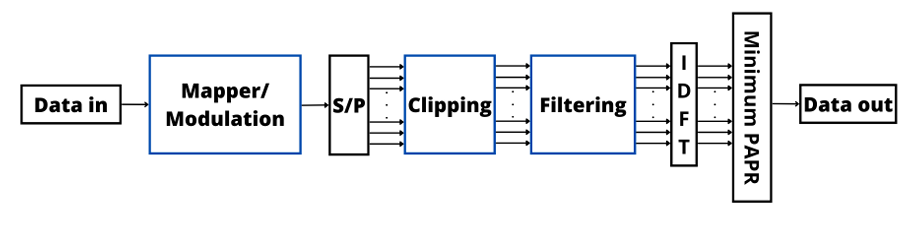
\includegraphics[width=0.75\linewidth]{Figures/OFDM_Refresher/clipping_filtering.png}
    \caption{Block diagram of an OFDM transmitter with clipping and filtering. The signal is clipped in the time domain, then filtered in the frequency domain to remove out-of-band distortion.}
\end{figure}

While clipping and filtering is simple to implement and requires no side information, it introduces in-band distortion (increasing BER) and out-of-band radiation.

\paragraph{Active Constellation Extension (ACE).}
ACE extends outer constellation points away from the decision boundaries to reduce peak power, without affecting BER.  No side information is required, as the extended points remain within their correct decision regions.

\begin{figure}[H]
    \centering
    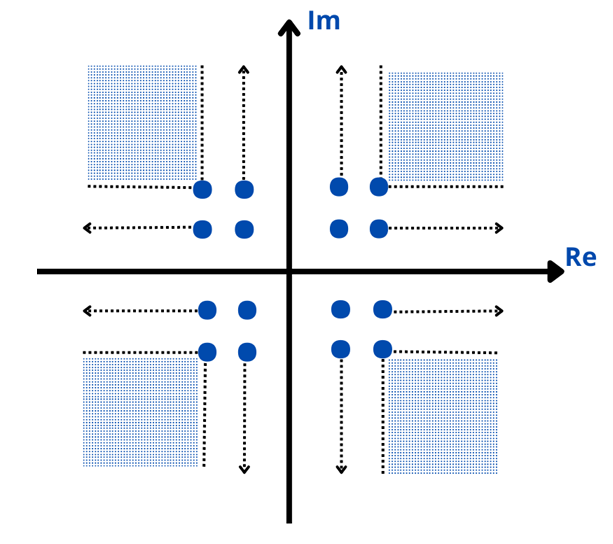
\includegraphics[width=0.55\linewidth]{Figures/OFDM_Refresher/ace_constellation.png}
    \caption{Active Constellation Extension for 16-QAM. Outer constellation points are extended into feasible regions (shaded), reducing the PAPR without crossing decision boundaries.}
\end{figure}

\paragraph{Tone Reservation (TR) and Tone Injection (TI).}
TR reserves a set of subcarriers exclusively for peak-cancelling signals, while TI adds carefully designed tones to the data subcarriers.  Both reduce PAPR without distorting data symbols, at the cost of reduced spectral efficiency (TR) or increased average power (TI).


\subsection{Signal Scrambling Methods}

Signal scrambling methods alter the signal representation \emph{without distortion} to find a low-PAPR version.

\paragraph{Partial Transmit Sequence (PTS).}
The input data block is partitioned into $V$ disjoint sub-blocks, each transformed by an IFFT independently.  The sub-blocks are then weighted by phase factors $b_v \in \{e^{j\phi} : \phi \in \Phi\}$ and summed. The phase combination yielding the lowest PAPR is selected for transmission.

\begin{figure}[H]
    \centering
    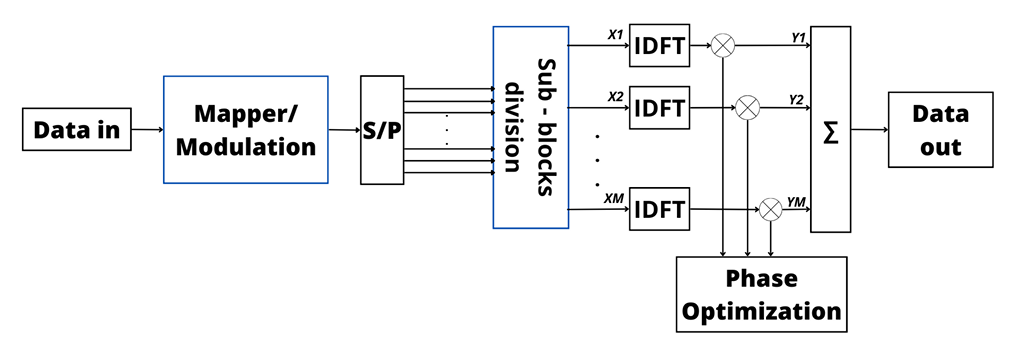
\includegraphics[width=0.85\linewidth]{Figures/OFDM_Refresher/pts_block_diagram.png}
    \caption{Block diagram of an OFDM transmitter with Partial Transmit Sequence (PTS).  The data is split into $V$ sub-blocks, each weighted by a phase factor after the IDFT. The combination with the lowest PAPR is transmitted.}
\end{figure}

\paragraph{Selected Mapping (SLM).}
Selected Mapping generates $U$ alternative representations of the same data block by multiplying the frequency-domain symbols with $U$ different phase sequences $\bm{\psi}_u$, each applied element-wise (Hadamard product):
\begin{equation*}
    \bm{X}_u = \bm{X} \odot \bm{\psi}_u,
    \qquad u = 1,\,2,\,\dots,\,U.
\end{equation*}
The corresponding time-domain candidates are obtained via the IFFT, and the candidate with the minimum PAPR is selected for transmission:
\begin{keyresult}
\begin{equation}
    \hat{u} = \arg\min_{1 \le u \le U}\;
    \mathrm{PAPR}\bigl(\bm{x}_u\bigr).
\end{equation}
\end{keyresult}
The receiver requires knowledge of which phase sequence was used, transmitted as $\lceil\log_2 U\rceil$ bits of \textbf{side information (SI)} per OFDM symbol.

\begin{figure}[H]
    \centering
    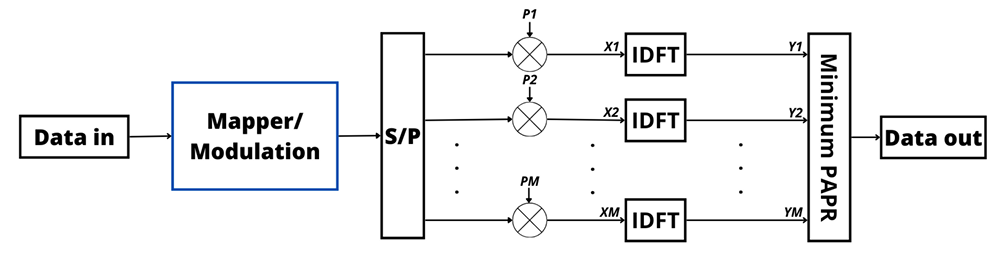
\includegraphics[width=0.75\linewidth]{Figures/OFDM_Refresher/slm_block_diagram.png}
    \caption{Block diagram of an OFDM transmitter with Selected Mapping (SLM). $U$ different phase sequences are applied to the frequency-domain data before the IDFT.  The candidate signal with the lowest PAPR is selected for transmission.}
\end{figure}

\paragraph{Interleaving.}
Multiple interleaving patterns are applied to the data, and the pattern producing the lowest PAPR is selected, analogous to SLM but using permutation rather than phase rotation.


\subsection{Comparative Summary}

\begin{table}[H]
    \centering
    \caption{Comparison of classical PAPR reduction techniques.}
    \label{tab:classical_comparison}
    \begin{tabular}{@{} l c c c c @{}}
        \toprule
        \textbf{Technique} & \textbf{BER Impact} & \textbf{Complexity} & \textbf{Side Info} & \textbf{Distortion} \\
        \midrule
        PTS          & None  & High     & Yes & No  \\
        SLM          & None  & High     & Yes & No  \\
        Interleaving & None  & Low      & Yes & No  \\
        Clipping     & Yes   & Low      & No  & Yes \\
        TI           & None  & High     & No  & No  \\
        TR           & None  & High     & Yes & No  \\
        ACE          & None  & Moderate & No  & No  \\
        \bottomrule
    \end{tabular}
\end{table}

\begin{figure}[H]
    \centering
    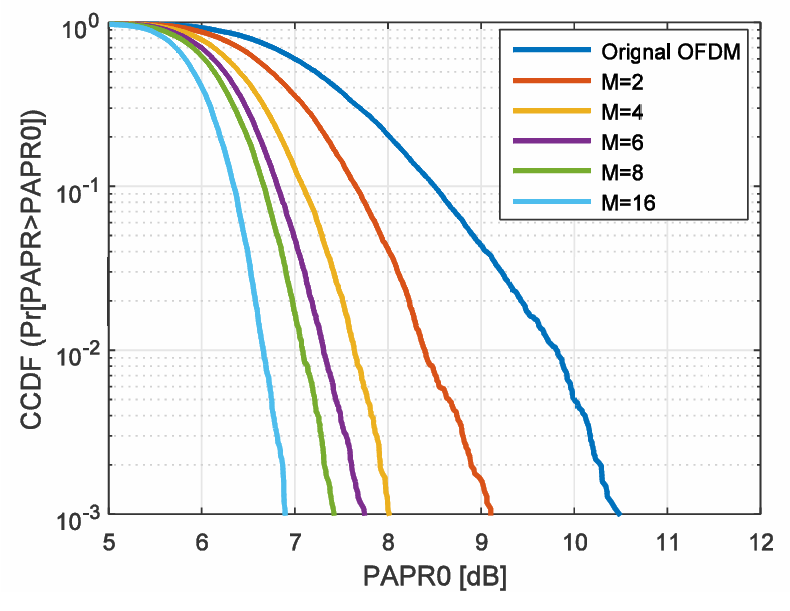
\includegraphics[width=0.55\linewidth]{Figures/OFDM_Refresher/slm_ccdf_varying_m.png}
    \caption{CCDF of PAPR for conventional SLM with different numbers of phase sequences $U$ ($N=128$, QPSK). Increasing $U$ improves PAPR reduction but with diminishing returns.}
\end{figure}


% ----------------------------------------------------------------------------
\section{Limitations of Classical Approaches}
\label{sec:classical_limitations}
% ----------------------------------------------------------------------------

Despite their effectiveness, classical PAPR reduction techniques suffer from three fundamental limitations that motivate the machine-learning approaches explored in subsequent chapters.

\textbf{Computational complexity.} Methods such as SLM and PTS require multiple IFFT operations per OFDM symbol. SLM requires $U$ full $N$-point IFFTs, yielding a per-symbol complexity of $\mathcal{O}(U \cdot N\log_2 N)$, which becomes prohibitive for large $N$ and $U$.

\textbf{Side information overhead.} SLM and PTS require transmitting $\lceil\log_2 U\rceil$ SI bits per symbol. These bits must be received error-free for correct decoding; an error in the SI bits causes the entire OFDM symbol to be decoded incorrectly.  Protecting SI bits typically requires additional channel coding, further reducing spectral efficiency.

\textbf{Blind detection difficulty.} Eliminating SI overhead through blind detection at the receiver requires $U$ full FFT operations per symbol, and decision metrics become unreliable at low SNR.  Blind detection remains an open problem, particularly well-suited to machine-learning-based solutions.


% ----------------------------------------------------------------------------
\section{Summary}
\label{sec:ch1_summary}
% ----------------------------------------------------------------------------

This chapter established the OFDM signal model, defined the PAPR problem and its implications for power amplifier efficiency, and surveyed the landscape of classical PAPR reduction techniques.  The three core limitations identified --- computational complexity, side information overhead, and blind detection difficulty --- define the design objectives for the deep learning-based approach presented in the following chapter, where a jointly trained autoencoder replaces the multi-IFFT search with a single neural network forward pass and eliminates the need for side information entirely.
